\documentclass[12pt,]{article}
\usepackage{graphicx}
\usepackage{tikz}
\usetikzlibrary{shapes.geometric, arrows}

\title{Sprawozadanie lernicng}
\author{Tymon Łazowy}
\date{123,2123,12}


\tikzstyle{startstop} = [ellipse, rounded corners, minimum width=2cm, minimum height=1cm,text centered, draw=black,thick,fill=red!0]

\tikzstyle{io} = [trapezium,trapezium stretches=true,trapezium left angle=70,trapezium right angle=110,thick,minimum width=2cm,minimum height=0.85cm, text centered, draw=black,fill=blue!0]

\tikzstyle{process} = [rectangle,minimum width=3cm,minimum height=0.85cm,text centered,text width=3cm,draw=black,thick,fill=orange!0]

\tikzstyle{decision} = [diamond,minimum width=1cm, minimum height=1cm, text centered, draw=black, fill=green!0,thick]

\tikzstyle{arrow} = [thick,->,>=stealth]

\begin{document}

\begin{figure}
    \centering  
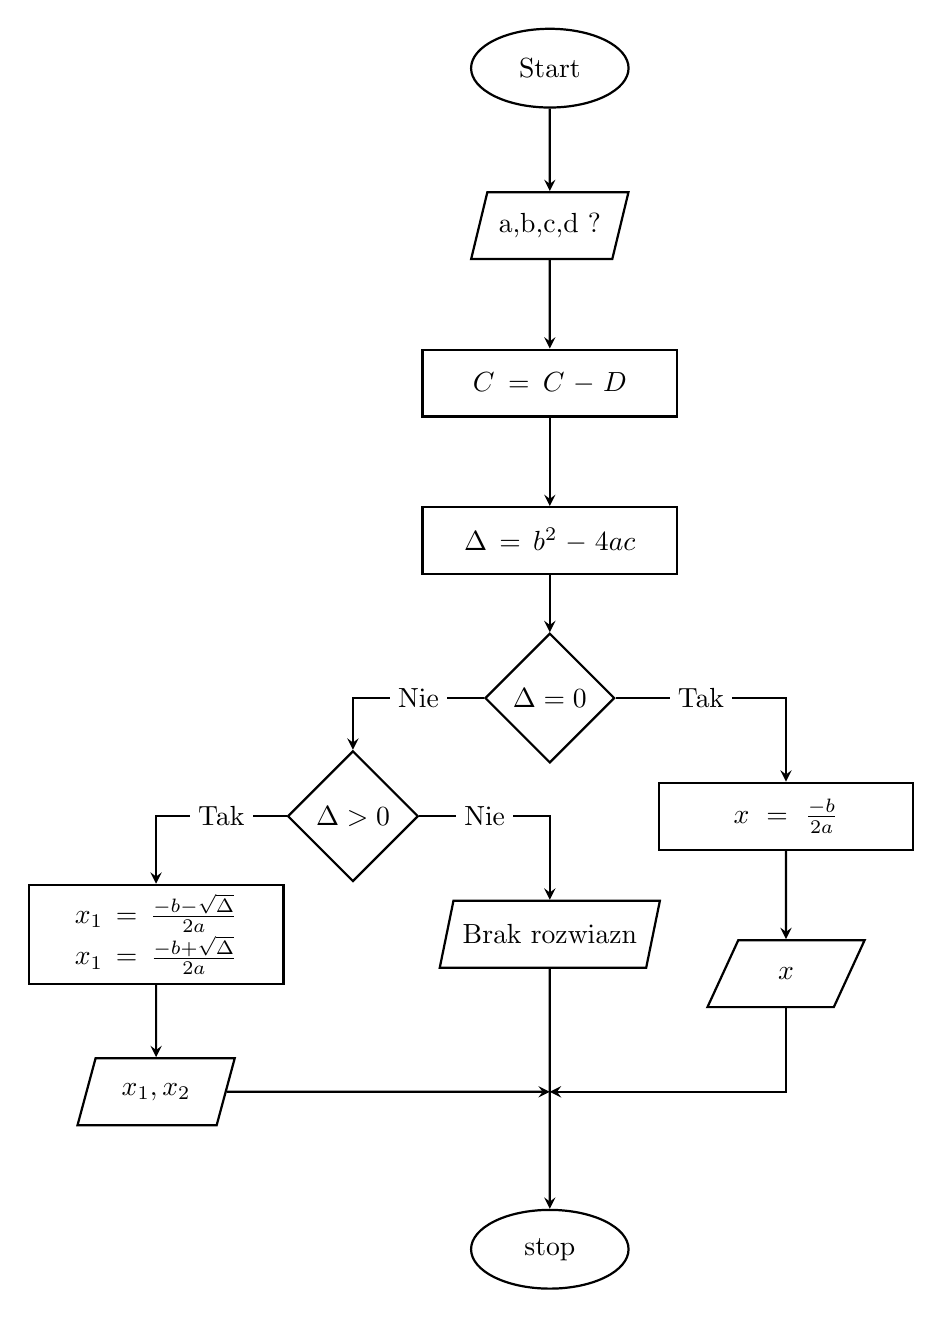
\begin{tikzpicture}[node distance=2cm]

\node (start) [startstop] {Start};
\node (in1) [io, below of=start] {a,b,c,d ?};
\node (pro1) [process, below of=in1] {$C=C-D$};
\node (pro2) [process, below of=pro1] {$\Delta=b^2-4ac$};
\node (dec1) [decision, below of=pro2,] {$\Delta=0$};
\node (tak1) [process, right of=dec1, xshift=1.0cm, yshift=-1.5cm] {$x=\frac{-b}{2a}$};
\node (out1) [io, below of =tak1]{$x$};
\node (dec2) [decision, left of=dec1, xshift=-0.50cm, yshift=-1.5cm] {$\Delta>0$};
\node (nie2) [io, right of=dec2, xshift=0.50cm, yshift=-1.5cm] {Brak rozwiazn};
\node (tak2) [process, left of=dec2, xshift=-0.50cm, yshift=-1.5cm] {$x_1=\frac{-b-\sqrt{\Delta}}{2a}$     $x_1=\frac{-b+\sqrt{\Delta}}{2a}$};
\node (out2) [io, below of =tak2]{$x_1,x_2$};
\node (meeting)[coordinate,below of =nie2]{};
\node (stop) [startstop, below of =meeting, yshift=0]{stop};

\draw [arrow] (start) -- (in1);
\draw [arrow] (in1) -- (pro1);
\draw [arrow] (pro1) -- (pro2);
\draw [arrow] (pro2) -- (dec1);
\draw [arrow] (tak1) -- (out1);
\draw [arrow] (tak2) -- (out2);
\draw [arrow] (nie2) -- (stop);
\draw [arrow] (out2) -- (meeting);
\draw [arrow] (out1) |-(meeting);
\draw[arrow] (dec1) -| (dec2) node[pos=0.25,fill=white,inner sep=3]{Nie};
\draw[arrow] (dec1) -| (tak1) node[pos=0.25,fill=white,inner sep=3]{Tak};
\draw[arrow] (dec2) -| (tak2) node[pos=0.25,fill=white,inner sep=3]{Tak};
\draw[arrow] (dec2) -| (nie2) node[pos=0.25,fill=white,inner sep=3]{Nie};

\end{tikzpicture}
    \caption{Funkcja kwadratowa}
    \label{flow2}
\end{figure}
\end{document}

